\section{Introduction}
\subsection{Context}
Urbanization is one of the most transformative trends of the 21st century. Although, urban areas only occupy 2\% of the world’s surface, by 2050, the percentage of urban population is expected to reach 68\% and to nearly double in size. Virtually, all future population growth will be absorbed by cities. Human activity in urban areas consume 75\% of global energy and are the place where 80\% of the C02 emissions are produced \cite{UN2018}. In this context, it has never been more evident that 
%
    \begin{quote} 
    The battle for sustainable development will be won or lost in cities \cite{UnitedNations}.
    \end{quote}\par
%
At first glance, the fact that by focusing on solutions on cities to revert current trends, might seem an easy task to accomplish, but the truth is the complete opposite; there are hundreds if not thousands of caveats that undermine the task, makes it one of the challenges of our era. To begin with, our concept of what a city is might not be a unified vision. We might tend to believe that most humans live in world cities such as London, Paris or Berlin, but in fact the population distribution by city sizes shows that we live in a more heterogeneous world; ( see \ref{fig:pop_dist}).\par

\begin{figure}[hbt!]
    \centering
    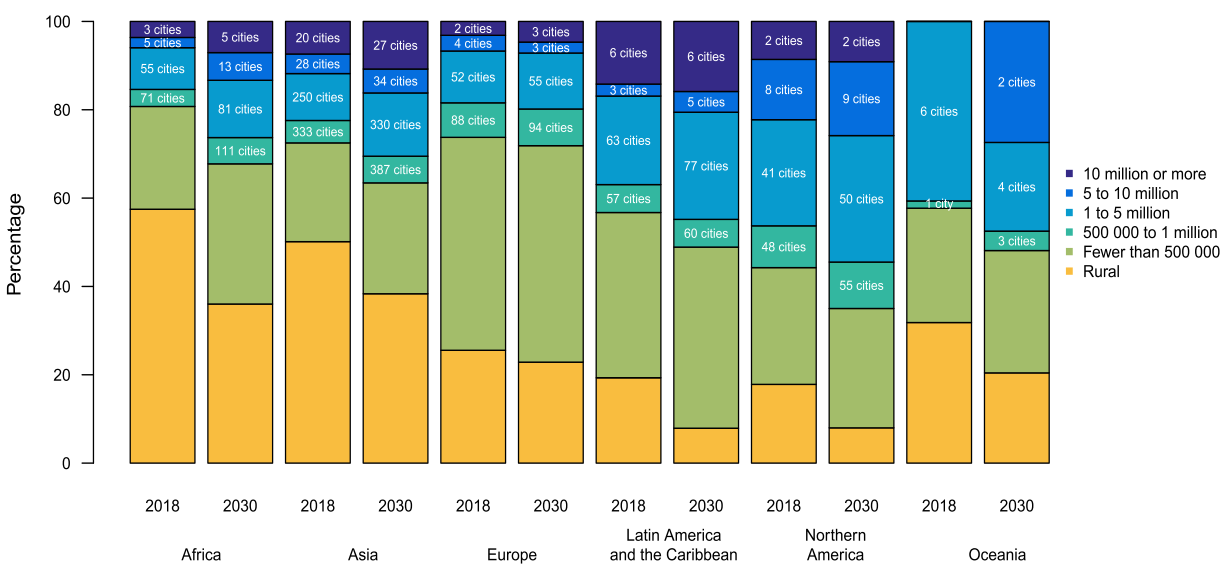
\includegraphics[width=0.85\textwidth]{Imgs/1_pop_dist.PNG}
    \caption{Population distribution by size class of settlement* and region, 2018 and 2030}
    \label{fig:pop_dist}
\end{figure}
 
Diversity in city sizes imply that there are other sources of heterogeneity such as context, socio-demographic characteristics, local capacities, and so forth. As can be obvserved in \ref{fig:pop_dist} there is a significant amount of citizens living in emerging cities. Consequently, it would be important for emerging cities to catch up with strategies and capacities of top-tier cities, to face global challenges. 
(Reinforce these concepts with proper citations). \par


In second place, there is no agreement or unified definition of what a city is. Throughout history, there has been significant efforts to understand and delimit the boundaries of cities. For certain, this is a highly contested arena with ongoing improvements and the definition of how an urban system is defined depends on what the focus of the study is. For instance, when dealing with municipal finances, research tends to use an administrative definition of the city; when analyzing job accessibility, the city is defined depending on the population  the case of accessibility of jobs, the definition of what a city is depends on the population travel patterns; finally but not least, research done in urban expansion tend to look at the physical aspects and satellite images are used to delimit the city. 
At some point, we might come to realize that there is no single definition of a city; its a social construction, bounder less system, an object that will need to be defined in every work, depending on the study focus. In this sense, this work will deal with the concept of City-Regions, as a physical bounder less definition of human settlements. Concepts such as city, functional urban area (FUA) or urbanity will be used interchangeably in hat follows. 

(Reinforce these concepts with proper citations) \par



\begin{figure}[hbt!]
    \centering
    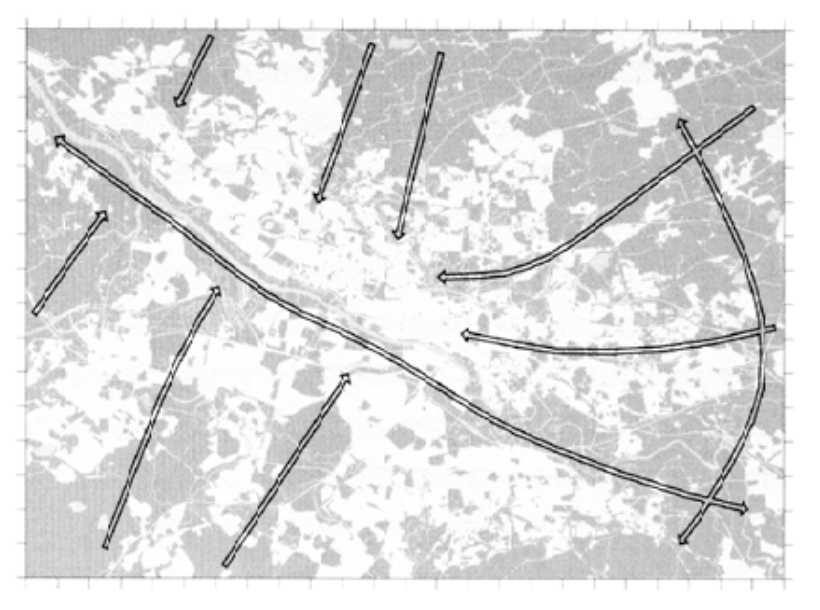
\includegraphics[width=0.5\textwidth]{Imgs/2_fua.PNG}
    \caption{Hildebrand Frey. Designing the City. Towards a more Sustainable Urban Form. Page 161.]}
    \label{fig:fua}
\end{figure}

Besides the fact that for the first time we are living in an urban world, it seems also important to highlight that we are living in a highly connected world. Since 2008, the number of devices connected to the internet has surpassed the number of humans on it. It is estimated that by 2020, 50 Billion devices will be actively connected to the web. In the context of city diversity, and lack of city boundaries, this fact becomes disruptive as there is an opportunity for sensing what is happening in human settlements disregards of the size, shape or boundary.\par


\begin{figure}[ht!]
    \centering
    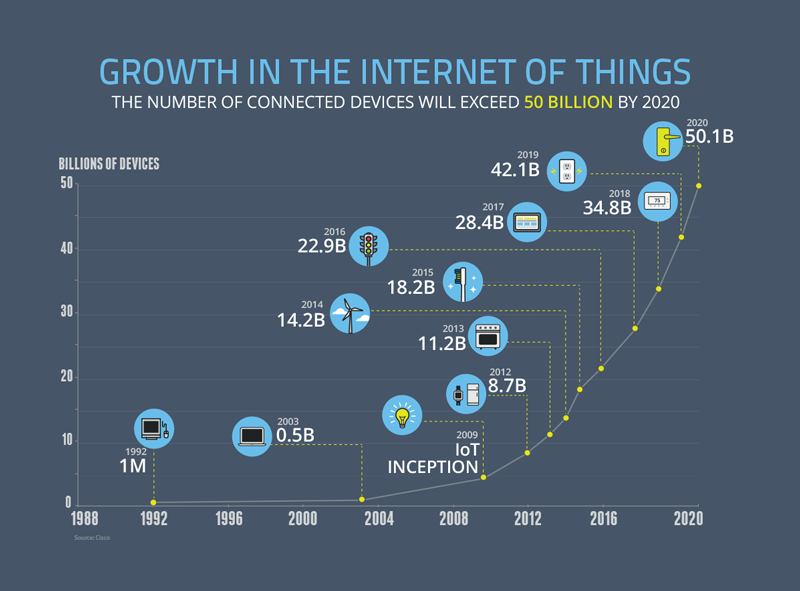
\includegraphics[width=0.5\textwidth]{Imgs/3_iot.png}
    \caption{Connected devices. IoT by 2020}
    \label{fig:iot}
    \url{https://www.ncta.com/whats-new/behind-the-numbers-growth-in-the-internet-of-things-2}
\end{figure}

\subsection{Motivation}
Above all this Phd project is steered by the outcomes of the UN Sustainable Development Summit in 2015. The process initiated back in 2013 culminated in the adoption of the 2030 Agenda for Sustainable Development, with specific focus on 17 Sustainability Development Goals (SDGs). \par

Together with the 17 Goals, a set of sub-goals and 244 performance indicators were agreed upon \cite{UN2017}. As pointed out above, cities (of all sizes) are found to be important pieces in the sustainable development game. Its relevance has been detailed in the Sustainable Development Goals (i) 11: make cities and human settlements inclusive, safe, resilient and sustainable and (ii) 12: Ensure sustainable consumption and production patterns. \par

For instance, SDG 11 contains 7 sub-goals (plus 3) and its progress is being monitored by 15 Key Performance Indicators (KPIs). Sub-goal 11.6 commits to reduce the adverse per capita environmental impact of cities, including by paying special attention to air quality and municipal and other waste management by 2030; and its evolution is being tracked by the KPI 11.6.1: The Proportion of urban solid waste regularly collected and with adequate final discharge out of total urban solid waste generated, by cities. The structure of Goal, - Sub goal and KPI(s) is repeated for every SDG and they are self-defined by the UN as

\begin{quote}
    blueprint to achieve a better and more sustainable future for all.
    \url{https://www.un.org/sustainabledevelopment/sustainable-development-goals/}
\end{quote}
\par

Although its controversy in Business Management, the idea that ‘one cannot manage, what is not measured’ is now taken as granted. Significant amount research contributions have been trying to understand the importance of measuring performance in both, private and public institutions. There is a tradition that argues that metrics are negative and perceive
\begin{quote}
    Quantitative performance measurements-whether single, multiple, or composite-are seen to have undesirable consequences for over-all organizational performance. The complexity of large organizations requires better knowledge of organizational behavior (...)
    \cite{Ridgway2016}
\end{quote}
In another philosophical tone, the value of indicators is acknowledged, but understanding that ‘performance measurement is not an end in itself’ and they could be used to (i) Learn what is working and what is not and (ii) Improve by identifying what would be done differently to improve \cite{Behn2003}.
In this project the value of the SDGs and KPIs is recognized as an important step towards building more sustainable and livable places. Setting goals and measuring them is one the first stages to improve performance, but to meet these targets another tool is needed. Planning (and execution) become crucial. P. Hall \cite{Hall1992} define 

\begin{quote}
    Planning as a general activity is the making of an orderly sequence of action that will lead to the achievement of a stated goal(s)’ and motivates to question what the strategies and actions are needed to achieve the SDGs. More specifically, it is important to acknowledge that these events and activities happen somewhere in the territory which also need to be planned. (...)\par
    Planning with a spatial, or geographical, component, in which the general objective is to provide for a spatial structure of which in some way is better than the pattern that would exist without planning. Urban planning (or regional planning) is a special case of general planning, which does include the plan-making, or representational, component
    
\end{quote}


\subsection{Challenge}
The importance of the SDGs and its KPIs is recognized as a step forward to meet the global sustainability. Yet the gap between indicators and how the planning of city-regions is done needs to be bridged. There is a challenge rised by the SDG11, to build better human settelemnts, and this mean dealing with the spatially planning of places. In order to plan better city-regions there is a need of spatializing, modelling and understanding  how this information can be adequately incorporated into the different Planning Processes. \par

As described above, KPIs do not give information about the set of actions needed to create sustainable places or improve how resources can be used more efficiently. Studying and understanding the interaction between the indicators is crucial, but also where these events or actions happen (Space or Spatialization) is important and not trivial. \par

In order to meet the targets, it has never been clearer that spatial planning is necessary. In some urban domains such as transport, there has been long tradition of exploring the relation between land use, mobility and socio-economic activities. As a result of data availability and it's natural proximity to geography, transport systems have been spatially planned for long time. New data sources and technological innovation can contribute to enhance the study of space in other urban domains.
